\subsubsection{Business Layer}

\begin{figure}[H]
    \centering
    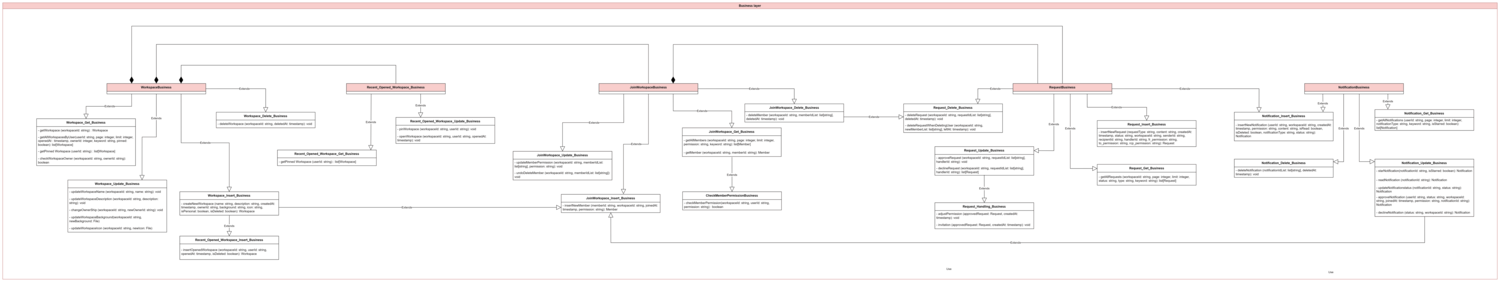
\includegraphics[ width = \linewidth]{Content/Phân tích và thiết kế hệ thống/documents/Sơ đồ lớp/images/Business layer/businessLayer.png}
    \vspace{0.5cm}
    \caption{Business Layer}
    \label{fig:Business Layer}
\end{figure}

Nhiệm vụ của tầng Business là phân tích những yêu cầu, xử lý logic nghiệp vụ và
gọi tới các đối tượng ở tầng Persistence để tương tác với cơ sở dữ liệu.

\begin{figure}[H]
    \centering
    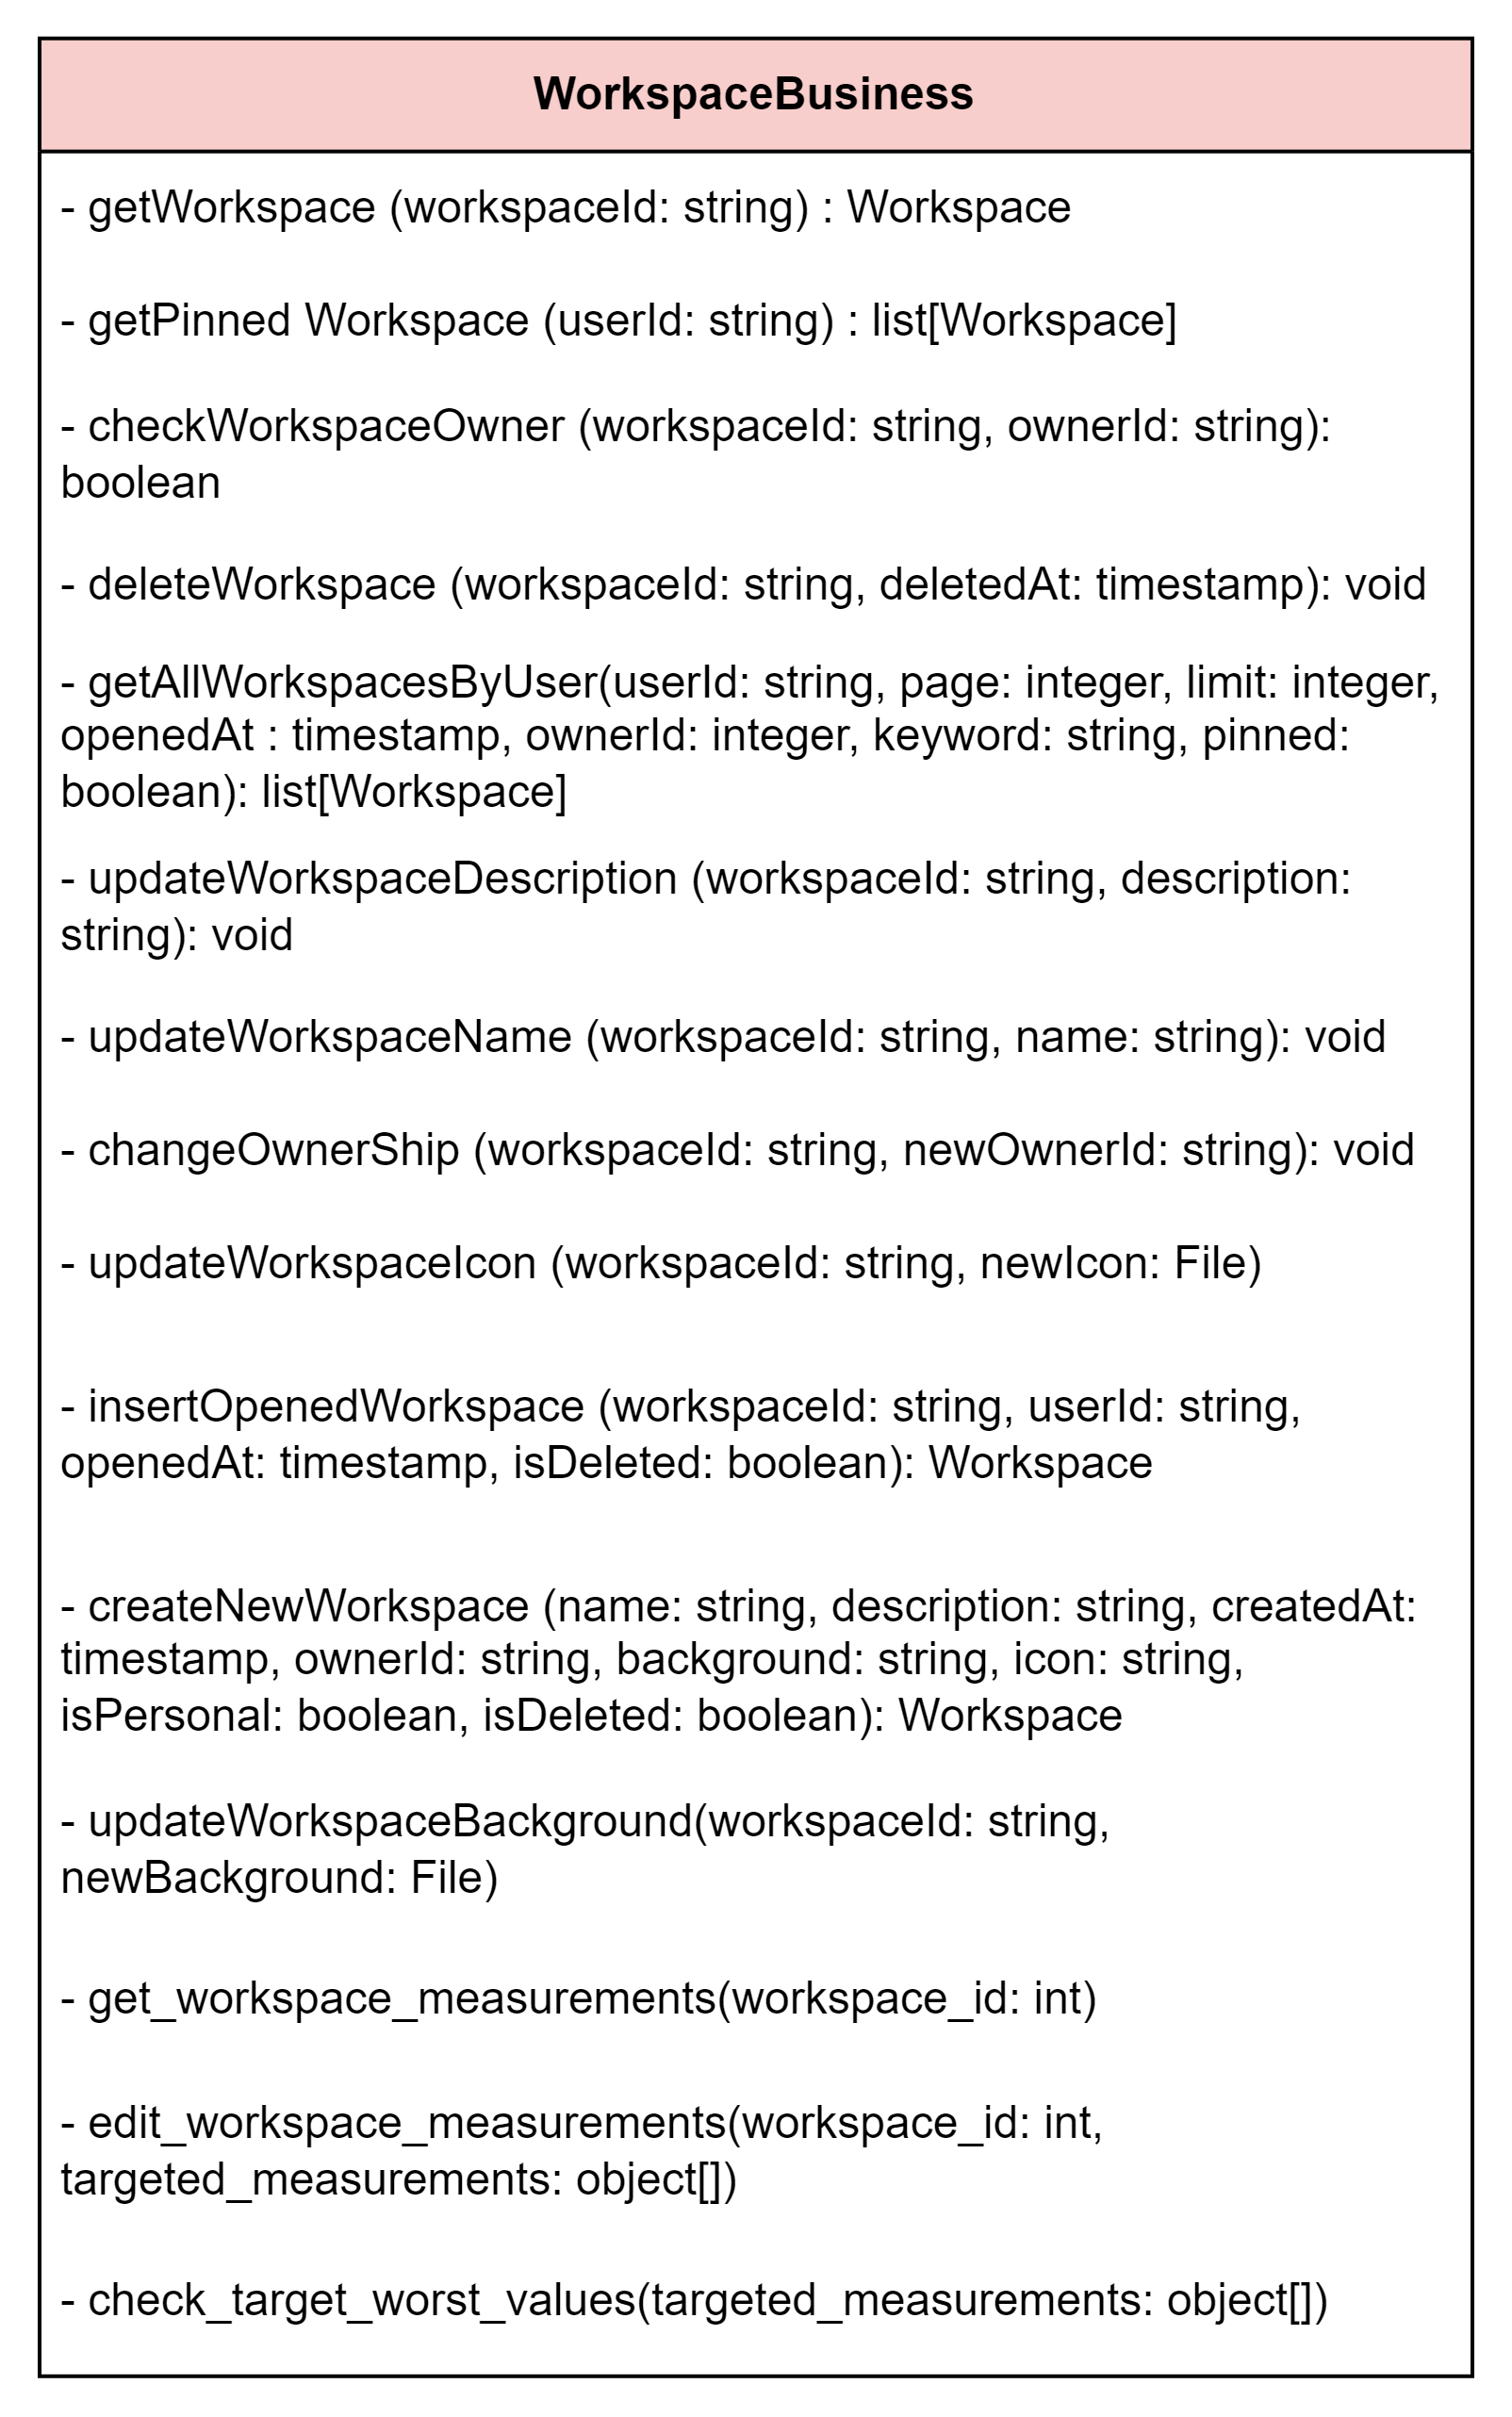
\includegraphics[ width = \linewidth]{Content/Phân tích và thiết kế hệ thống/documents/Sơ đồ lớp/images/Business layer/workspaceBusiness.png}
    \vspace{0.5cm}
    \caption{Workspace Business}
    \label{fig:Workspace Business}
\end{figure}

\begin{figure}[H]
    \centering
    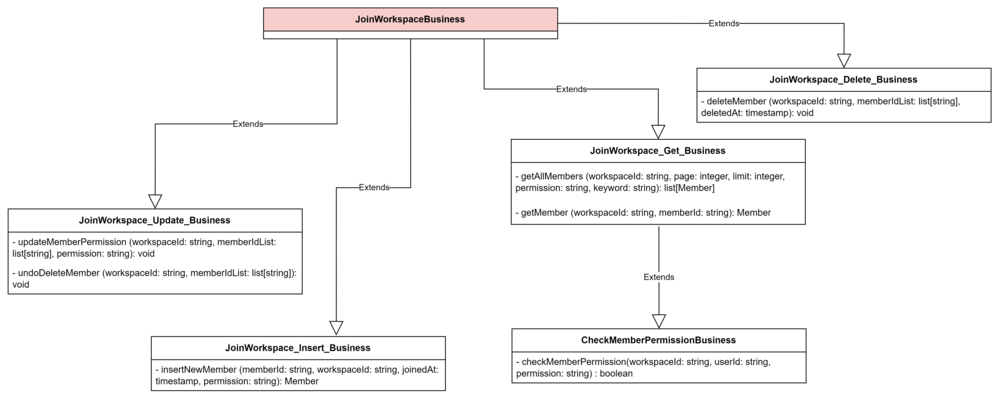
\includegraphics[ width = \linewidth]{Content/Phân tích và thiết kế hệ thống/documents/Sơ đồ lớp/images/Business layer/joinWorkspaceBusiness.png}
    \vspace{0.5cm}
    \caption{Join Workspace Business}
    \label{fig:Join Workspace Business}
\end{figure}

\begin{figure}[H]
    \centering
    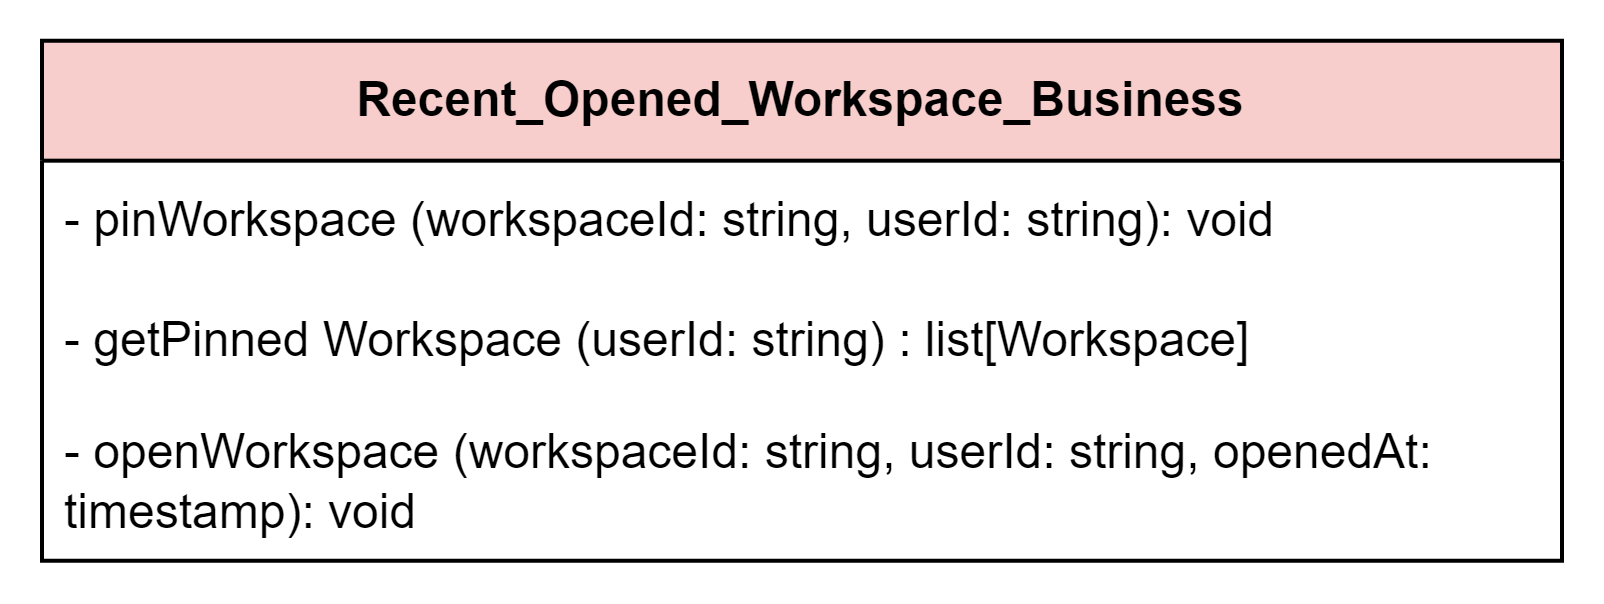
\includegraphics[ width = \linewidth]{Content/Phân tích và thiết kế hệ thống/documents/Sơ đồ lớp/images/Business layer/recentOpenedWorkspaceBusiness.png}
    \vspace{0.5cm}
    \caption{Recent Opened Workspace Business}
    \label{fig:Recent Opened Workspace Business}
\end{figure}

\begin{figure}[H]
    \centering
    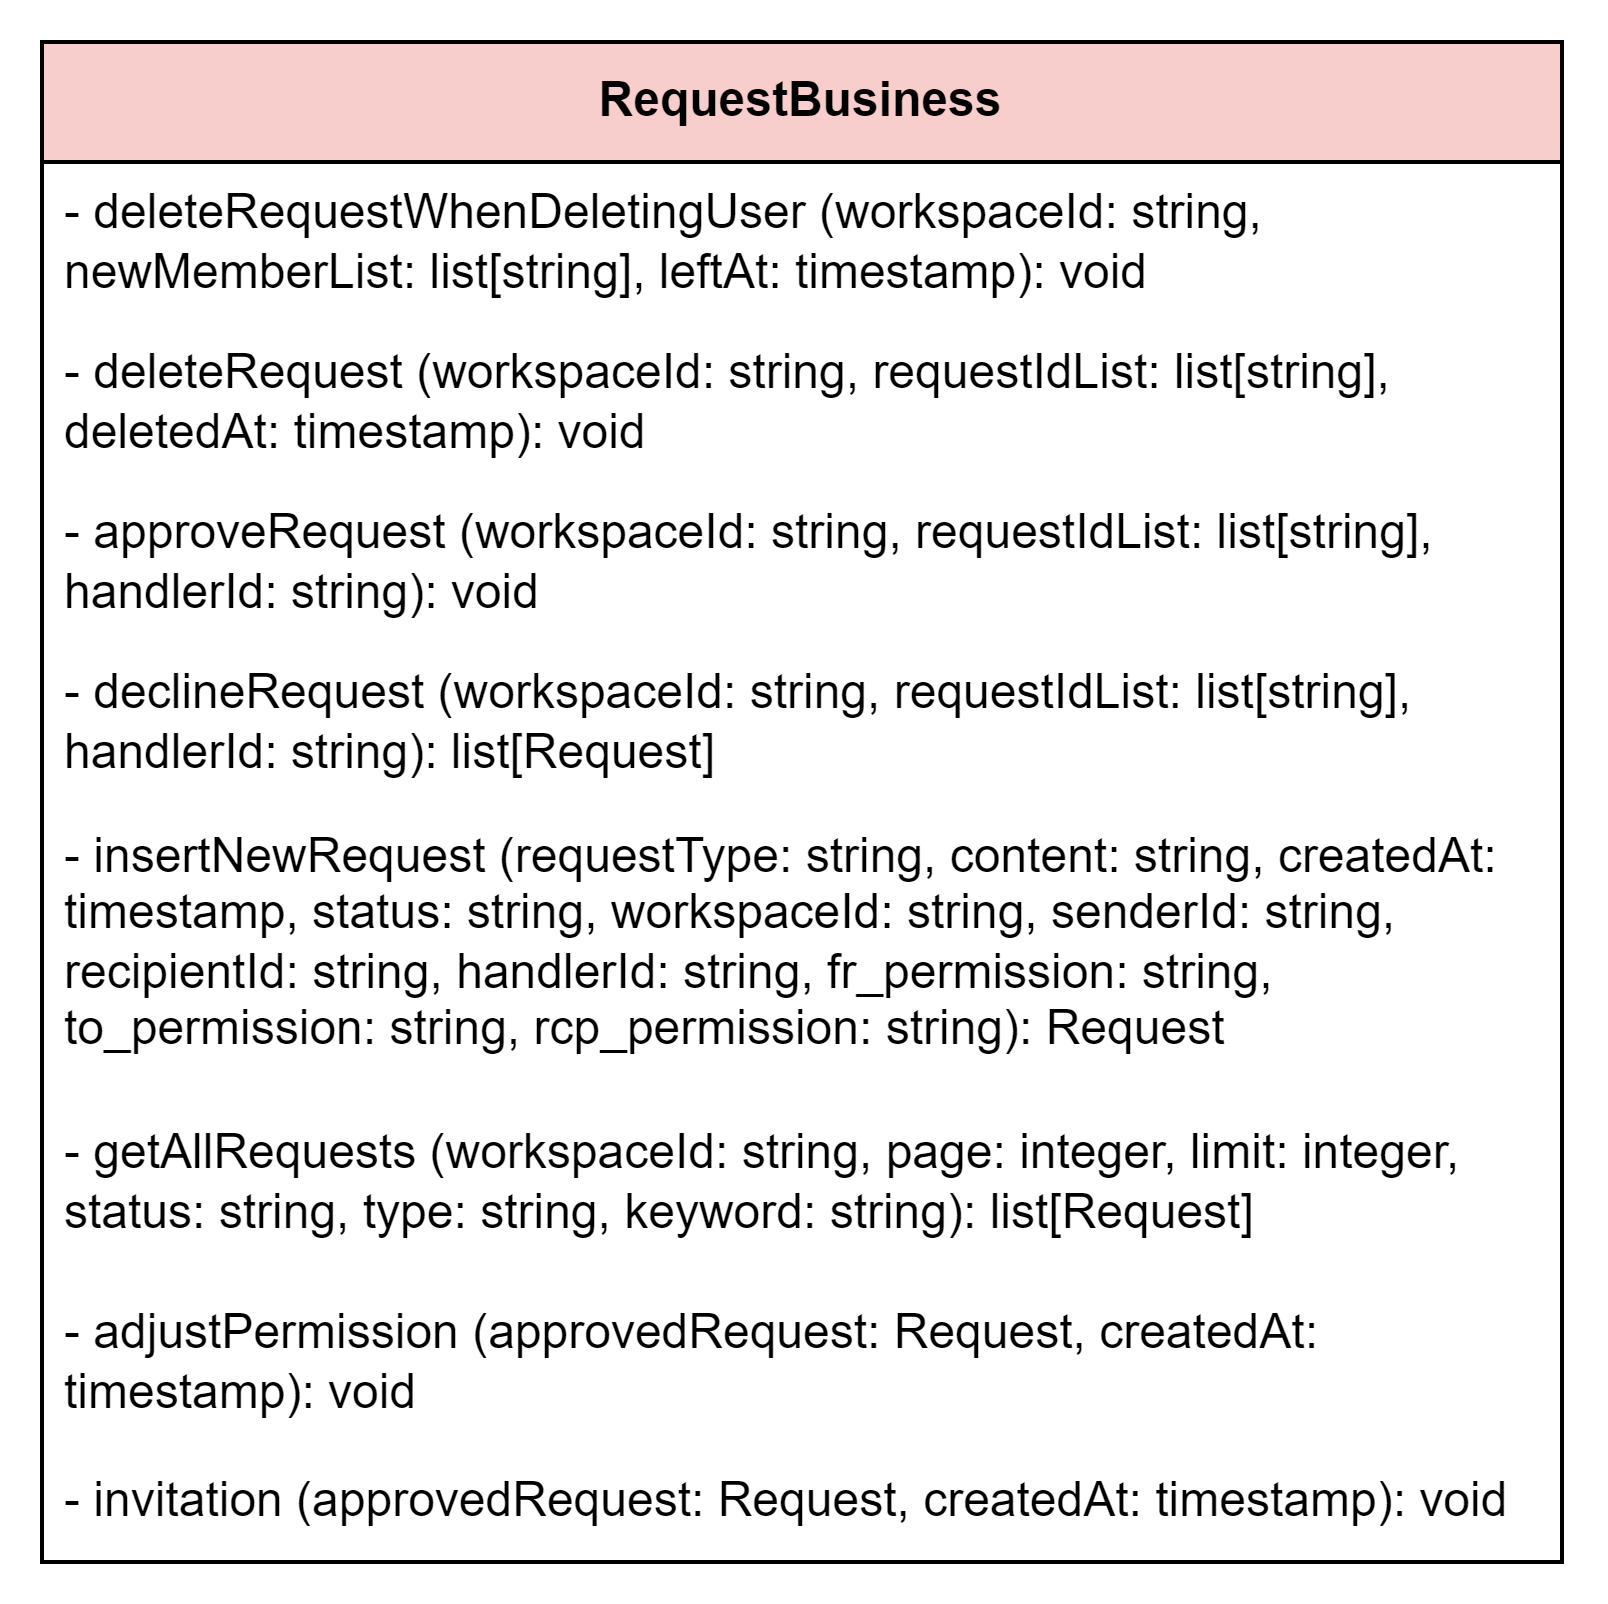
\includegraphics[ width = \linewidth]{Content/Phân tích và thiết kế hệ thống/documents/Sơ đồ lớp/images/Business layer/requestBusiness.png}
    \vspace{0.5cm}
    \caption{Request Business}
    \label{fig:Request Business}
\end{figure}

\begin{figure}[H]
    \centering
    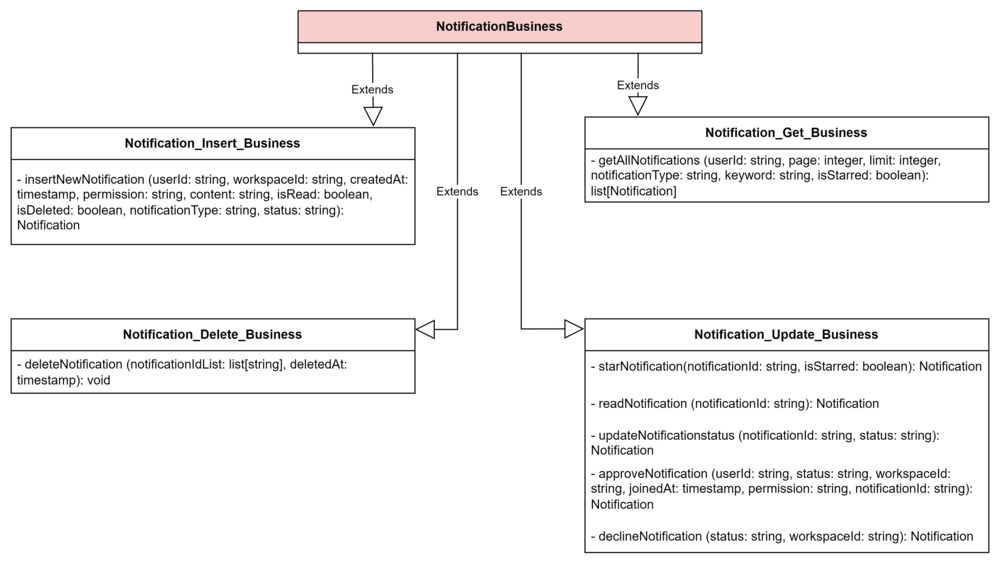
\includegraphics[ width = \linewidth]{Content/Phân tích và thiết kế hệ thống/documents/Sơ đồ lớp/images/Business layer/notificationBusiness.png}
    \vspace{0.5cm}
    \caption{Notification Business}
    \label{fig:Notification Business}
\end{figure}

